\documentclass[../HDF5_RFC.tex]{subfiles}

\begin{document}

\section{Multi-threaded tests}
\label{multithread}

\subsection{Integrating with HDF5's 'testframe' testing framework}

As developers will already be dealing with the difficulty of multi-threading in regards to both library
and test code development, the best approach to writing multi-threaded tests will be to integrate with
HDF5's 'testframe' testing framework (that is, include and use the functionality from \texttt{testframe.h} / \texttt{testframe.c}), simplifying portions of testing code and making multi-threaded tests consistent
with each other. As issues are found with adapting a multi-threaded test into this testing framework,
changes to the framework should be made to make the process easier for other tests in the future. Refer
to Appendix \ref{apdx:multithread_example} for an example of a skeleton for a multi-threaded test program
that integrates with the 'testframe' testing framework.

If a multi-threaded test program integrates with the 'testframe' framework, it should be sure to pass
the value \texttt{H5\_MULTITHREAD\_TEST} for the \texttt{TestFrameworkFlags} parameter when calling
\nameref{apdx:testframe_testinit}. This ensures that the testing framework can setup any state it needs
to for running multi-threaded tests. A multi-threaded test program then has two options for running
a multi-threaded test: by managing threading itself or by allowing the testing framework to manage
threading. When adding a test to the list of tests with \nameref{apdx:testframe_addtest}, the
\texttt{TestFlags} parameter can control this behavior. If the value \texttt{ALLOW\_MULTITHREAD} is
present in the flags specified in this parameter, the testing framework will use a set of threads it
creates internally to run the test. Otherwise, it is up to the test program to manage threading for
that particular test. See Appendix \ref{apdx:testframe_performtests} for more details.

\subsection{Allowing for a configurable number of threads}

Any multi-threaded HDF5 test program should allow for specifying a maximum number of threads to be
used within that program. While sub-tests of the test program may end up using less than the specified
number of threads, they should generally be designed to be flexible and also not impose a minimum
required number of threads (i.e., should be able to run with a single thread if need be). After integrating
with the 'testframe' testing framework, multi-threaded test programs will have the command-line option
\texttt{-maxthreads} that allows specifying the maximum number of threads the program can spawn in addition
to the main thread for the program. The test program can then call the \nameref{apdx:testframe_gettestmaxnumthreads} utility function to query this value and make adjustments at
run time. When a multi-threaded test program is running with a \texttt{TestExpress} value that indicates it should only perform smoke checks, it is recommended that the test program spawn a random number of threads
up to the maximum allowed in order to have better testing coverage of multi-threaded functionality.

\subsection{Error handling in multi-thread tests}

Similar to HDF5's parallel tests, handling errors in multi-threaded HDF5 tests will require careful design
from test authors to prevent hangs that starve out other tests\footnote{This is especially important for running CI on HPC machines, where jobs are typically run on debug queues that generally have around 30
minute allowances before a job is killed.}. When something fails in a multi-threaded HDF5 test, that
failure may need to be collectively communicated so that other threads can cleanup and exit the test.
Multi-threaded test authors are encouraged to:

\begin{enumerate}

    \item Minimize the number of synchronization points, where possible
    \item Avoid HDF5's typical \texttt{goto}-style error handling at synchronization points and instead
          capture a success or failure value that can be communicated between threads\footnote{Using
          mutual exclusion or atomic instructions to increment a shared variable on failure, then waiting
          on the result with a \texttt{pthread\_barrier\_wait()} call seems to be a rudimentary but
          sufficient approach} to ensure they collectively proceed or fail

\end{enumerate}

When the 'testframe' framework is allowed to run a test using its own internal threads, the framework
aggregates the pass/fail status of a test after all the threads have been joined. Using this approach
for a test may help to simplify error handling for test authors.

\subsection{Output from multi-threaded tests}

Similar to parallel HDF5 tests, multi-threaded HDF5 tests will also have issues with interleaved output
without careful consideration. Multi-threaded tests should:

\begin{itemize}

    \item Only print output from a single thread after choosing a "leader". A reasonable strategy would be
          to algorithmically pick a leader based on the "thread ID" that HDF5 chooses for the thread and
          stores in that thread's specific/local storage. Note that the 'testframe' framework also provides
          a "thread ID" value in the testing parameters passed to a test function.
    \item Use locking primitives or POSIX's \texttt{flockfile()} to prevent interleaving of output. Ideally
          this locking would eventually be integrated into the testing framework and exposed by utility functions to simplify the writing of testing code. Note that, even with this locking, output can become interleaved if it occurs across multiple \texttt{printf()}-like function calls; tests will need to either group all output from a thread into a single lock-unlock cycle (likely at the end
          of the test), or have some synchronization point between "rounds" of output from threads.
    \item Print output from threads into separate log files, where each file is solely owned by a single
          thread and is named based on some algorithmic strategy. While best left for debugging purposes
          only, this approach can be very useful for developers to reason about problems in multi-threaded tests.

\end{itemize}

Note that any output from the 'testframe' testing framework, such as the printing out of test names or information, should not occur in multiple threads simultaneously and so does not needed to be guarded
against by test programs integrated with this testing framework. The framework also provides several
macros that can be used to print output "correctly" in a multi-threaded test program (where "correctly"
usually means restricting output to the "main" thread).

\subsection{Organization and differentiation of tests}

Historically, integration tests have often not been written for new HDF5 features, with the vast majority
of the library's tests consisting of regression and unit/functionality tests. This often leads to surprising behavior in the future when different HDF5 modules interact. Due to the generally non-deterministic behavior when testing multi-threaded code, regression and unit tests alone will likely be insufficient for finding issues in multi-threaded HDF5; differences in application timing across platforms alone can be enough for specific problematic behaviors to not be reproduced. The most useful tests will rather be unit and
integration tests that focus on testing the functionality of a specific module of HDF5 (e.g., H5I, H5P,
etc.), as well as testing the interactions between different modules.

Therefore, this document proposes that some level of organization should be introduced to the HDF5 library's
testing directory structure as multi-threaded tests are added. At a minimum, a new directory\footnote{Suppose this directory is called 'threads' for the time being} should be created under the library's \texttt{test} directory; one may also be created under the \texttt{testpar} directory for future multi-threaded parallel tests if necessary. Under this new directory should be further sub-directories that separate unit tests
from integration tests, where the unit tests sub-directory has multiple sub-directories, one for each HDF5 module tested, and the integration tests directory has sub-directories based on the specific "feature" (or combination of modules) being tested. The hope is that this organization structure will encourage developers to:

\begin{itemize}

    \item Place their unit tests in the "correct" location, rather than spending time trying to determine if
          there is an existing test file their test should be placed in, or if a new test file should be
          created
    \item Be able to glance at the integration tests directory and quickly determine which modules need to
          be considered when it comes to cross-module interactions

\end{itemize}

Over time, this organization could also be applied to the library's existing serial tests as well. Figure \ref{fig:mt_test_dirs} is a visualization of what this would look like.

\begin{figure}
    \centering
    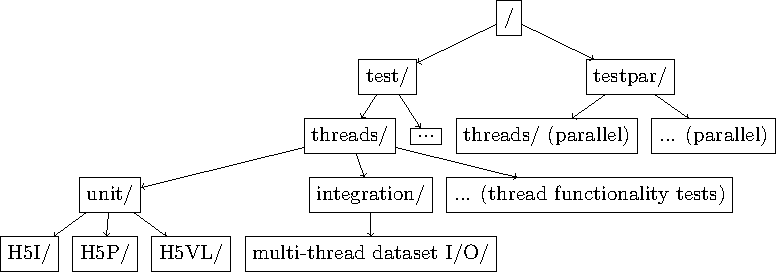
\includegraphics[width=0.8\linewidth]{images/MT_test_dirs.pdf}
    \caption{Organization of HDF5 multi-threaded tests}
    \label{fig:mt_test_dirs}
\end{figure}

\end{document}